\documentclass[main.tex]{subfiles}

\begin{document}
\subsection{Layered Architecture}
본 Database Management System (DBMS)의 전반적인 구조는 다음과 같다.

\begin{figure}[h]
	\centering
	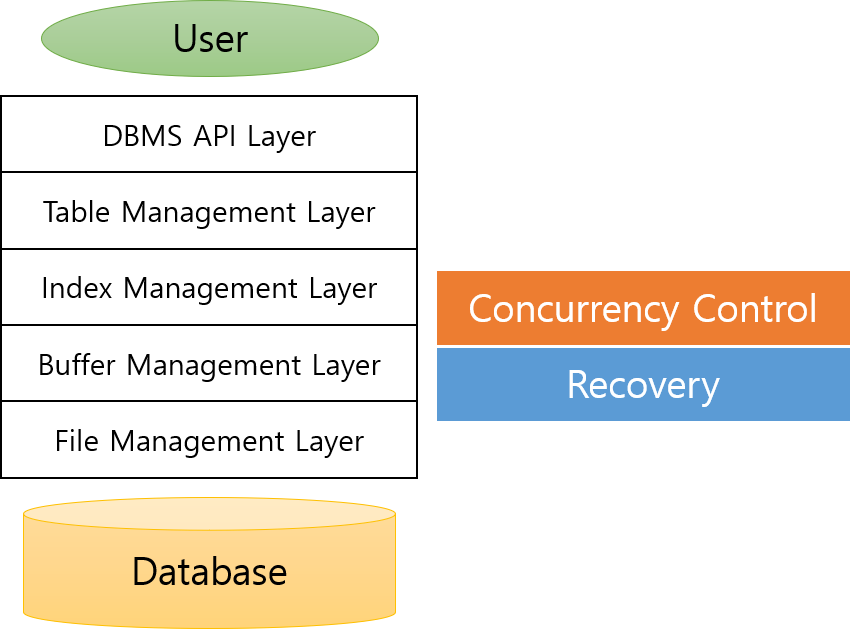
\includegraphics[width=0.7\textwidth]{images/layered/layered_architecture.png}
	\caption{Layered Architecture}
\end{figure}

\subsubsection{DBMS API Layer}
\begin{table}[!htb]
	\begin{tabularx}{\textwidth}{|l|X|}
		\hline
		\textbf{File} & dbapi.h dbapi.cpp \\
		\hline
		\textbf{Purpose} & 사용자에게 database를 수정, 조회 및 transaction processing engine에 접근하는 interface를 제공해준다.
		Table에 대해 insert, delete, update, find 연산 등 table에 관련한 작업은 \texttt{Table Management Layer}를 통해 수행한다.
		반면 transaction의 begin, commit, abort 작업은 \texttt{Transaction Manager}를 통해 수행한다. \\
		\hline
	\end{tabularx}
\end{table}


\subsubsection{Table Management Layer}
\begin{table}[!htb]
	\begin{tabularx}{\textwidth}{|l|X|}
		\hline
		\textbf{File} & table.h table.cpp \\
		\hline
		\textbf{Class} & TableManager Table \\
		\hline
		\textbf{Purpose} & 각 table 별로 테이블의 이름 및 파일 포인터를 저장 및 관리하며, \texttt{DBMS API Layer}와 \texttt{Index Management Layer} 간의 연결을 담당한다. \\
		\hline
	\end{tabularx}
\end{table}

\newpage
\subsubsection{Index Management Layer}
\begin{table}[!htb]
	\begin{tabularx}{\textwidth}{|l|X|}
		\hline
		\textbf{File} & bpt.h bpt.cpp \\
		\hline
		\textbf{Class} & BPTree \\
		\hline
		\textbf{Purpose} & 주어진 key에 대응되는 record를 빠르게 찾기 위한 access method를 제공하며, B+Tree를 이용해 구현하였다. \\
		\hline
	\end{tabularx}
\end{table}

\paragraph{Implementation}
B+Tree는 Amittai Aviram의 코드\footnote{Source Code: http://www.amittai.com/prose/bpt.c}를 C++로 포팅하였다.
별도의 state를 가지지 않기 때문에 모든 manager 중 유일하게 singleton class가 아니다.

\paragraph{Optimization}
원본 코드는 key를 찾을 때 linear search를 하였다. 하지만 본 DBMS에서는 internal page의 경우 key의 개수가 248개에 달해 linear search는 비효과적일 수 있다.
page 내부에서 key는 정렬된 상태를 유지하기 때문에 binary search의 도입을 고려할 수 있었으며, 두 방식의 성능을 비교한 결과 다음의 결과가 나왔다.

\begin{figure}[!htb]
	\centering
	\subfloat[100,000 times insert]{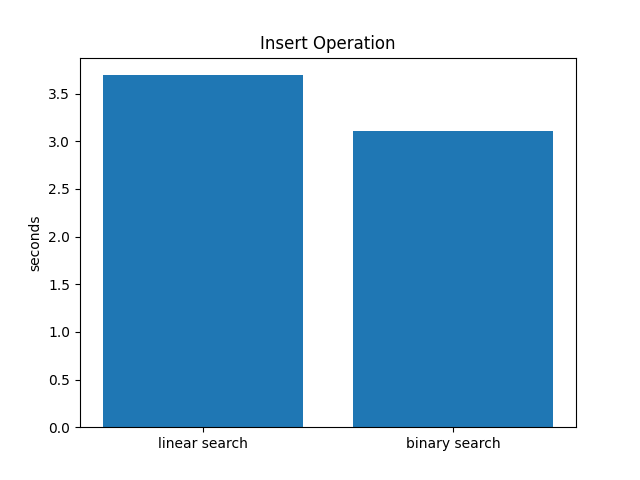
\includegraphics[width=0.48\linewidth]{images/layered/index_perf_insert_operation.png}}
	\subfloat[100,000 times find]{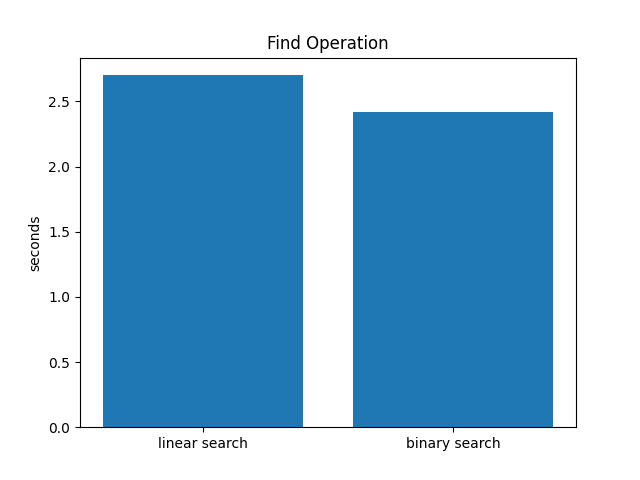
\includegraphics[width=0.48\linewidth]{images/layered/index_perf_find_operation.png}}
	\caption{Performance test for linear search and binary search}
\end{figure}

\subsubsection{Buffer Management Layer}
\begin{table}[!htb]
	\begin{tabularx}{\textwidth}{|l|X|}
		\hline
		\textbf{File} & buffer.h buffer.cpp page.h page.cpp \\
		\hline
		\textbf{Class} & BufferManager BufferBlock Page \\
		\hline
		\textbf{Purpose} & caching을 통해 메모리에 비해 느린 stable storage의 I/O 비용을 줄이고자 도입되었다. \\
		\hline
	\end{tabularx}
\end{table}

\paragraph{LRU Policy}
Doubly linked list를 이용해 LRU policy를 구현했다. page를 \texttt{Buffer Management Layer}에 요청하면 그에 해당하는 buffer block의 link를 끊고 tail에 insert 한다. 따라서 최근 요청된 buffer block일수록 linked list의 tail 쪽에 위치하고, 마지막 요청이 오래전일수록 head 쪽에 위치하게 된다. 따라서 eviction이 일어날 때는 head부터 victim을 찾는다.

\paragraph{Pin Management}
생성된 곳과 파괴하는 곳은 같아야 한다는 원칙에 따라 pin count의 관리는 모두 \texttt{Buffer Management Layer}에서 처리된다. 이러한 방법을 채택함으로써 pin count를 잘못 관리하여 생기는 버그의 근본 원인을 제거할 수 있다. 이러한 구현을 위해 요청한 측에 Page를 바로 주는 것이 아니라, 요청하는 쪽에서 Page를 바탕으로 어떠한 작업을 할지를 lambda expression으로 \texttt{Buffer Management Layer}에 제공하면 \texttt{Buffer Management Layer}에서 해당 작업을 실행하게 하는 방식으로 구현되었다. pseudo-code는 다음과 같다.

\begin{algorithm}
	\caption{Do work with Buffer Management Layer}
	\begin{algorithmic}
		\Function{DoWork}{table id, page id, $\lambda$}
		\Comment{$\lambda$는 page를 가지고 할 일}
		
			\State page = BufferManager.GetPage(table id, page id)
			\State page.pincount $\gets$ page.pincount $+ 1$
			
			\State result = $\lambda$(page)
			
			\State page.pincount $\gets$ page.pincount $- 1$
			
			\State \Return{result}		
		\EndFunction
	\end{algorithmic}
\end{algorithm}

\paragraph{Pinning Timing}
pin을 하는 시점은 선제적으로 필요한 모든 page에 대해 거는 방식과 필요할 때마다 pin을 하는 방식 중 후자를 채택했다. 이러한 방식을 채택함으로써 multi threading에서 \texttt{Buffer Management Layer}의 cache에 unpinned buffer block이 없어 다수의 worker가 대기하는 상황을 최소화 할 수 있을 것이다. 또한 4개 이상의 버퍼 크기에서는 완전히 동작하게 돼 memory가 작은 system에서도 돌아갈 수 있다.

\begin{table}[!htb]
	\centering
	\begin{tabularx}{.6\textwidth}{|c|X|}
		\hline
		\textbf{Operation} & \textbf{Maximum Pin Count} \\
		\hhline{|=|=|}
		Search & 1 \\
		\hline
		Insertion & 2 \\
		\hline
		Deletion (Coalesce) & 3 \\
		\hline
		Deletion (Redistribute) & 4 \\
		\hline
	\end{tabularx}
	\caption{각 operation별 maximum pin count}
\end{table}


\paragraph{Hash Table}
(table id, page id)에 해당하는 buffer block를 빠르게 찾기 위해 searching structure로 hash table을 두었다. Hash table의 구현체는 STL library의 unordered\_map을 이용하였다.
hashing function은 STL library에 있는 문자열에 대한 hashing function을 이용하여 만들었다.

\begin{algorithm}
	\caption{Hash function for tuple of (table id, page id)}
	
	\begin{algorithmic}[lines]
		\Function{Hash}{table id, page id}
		\State \Return {StringHashing(table id + "$|$" + page id)}
		\Comment{StringHashing은 STL library}
		\EndFunction
	\end{algorithmic}
\end{algorithm}

\newpage
\subsubsection{File Management Layer}
\begin{table}[!htb]
	\begin{tabularx}{\textwidth}{|l|X|}
		\hline
		\textbf{File} & file.h file.cpp \\
		\hline
		\textbf{Class} & FileManager File \\
		\hline
		\textbf{Purpose} & 각 table 별로 \texttt{Index Management Layer}가 활용할 page들을 stable storage에 저장 및 관리한다. \\
		\hline
	\end{tabularx}
\end{table}

\subsection{Data Flow}
본 section에서는 상황별로 data가 어떠한 방식으로 흘러가는지를 소개한다.

\subsubsection{Initialization and Shutdown}
\begin{figure}[h]
	\centering
	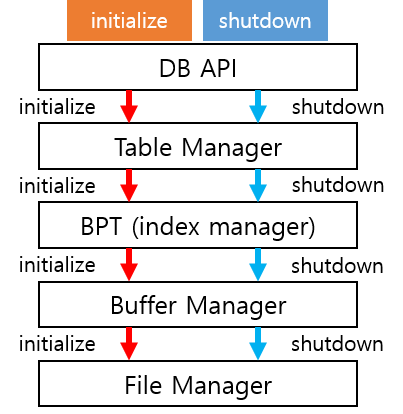
\includegraphics[width=0.5\textwidth]{images/dataflow/initialize_shutdown.png}
	\caption{Data flow in initialize and shutdown}
\end{figure}

\paragraph{Initialization} 
\texttt{DBMS API Layer}를 통해 사용자가 DBMS의 초기화를 요청하면 각 layer가 자신의 하위 layer의 초기화 메소드를 호출하는 방식으로 초기화를 진행한다.
하지만, 이때 하위 layer의 초기화가 완료되면 그 후에 자신의 초기화 작업을 수행하도록 하여, 최하단의 layer부터 상단의 layer의 순서대로 초기화됨을 보장한다.
또한 하위 layer에서 초기화 실패가 일어나면 그 이후의 layer들은 초기화가 진행되지 않으며 DBMS 초기화 작업이 실패했다는 신호를 보낸다.

\paragraph{Shutdown}
\texttt{DBMS API Layer}를 통해 사용자가 DBMS의 종료를 요청하면 각 layer가 하위 layer의 종료 메소드를 호출하는 방식으로 종료를 진행한다.
이때, 자신의 종료를 먼저 수행한 뒤 하위 layer의 종료를 수행하도록 하여, 최상단의 layer부터 시작하여 하단의 layer의 순서대로 초기화됨을 보장한다. 이는 위의 \textbf{initialization}의 순서와 반대이다.
또한 상위 layer에서 종료 실패가 일어나면 그 이후의 layer들은 종료를 수행하지 않으며 DBMS의 종료 작업이 실패했다는 신호를 보낸다.


\subsubsection{Open and Close Table}
Table을 열고 닫는 작업은 다수의 layer에 걸쳐 일어난다. 또한 table은 table id, file id 등을 가지고 있어야 하며, 각 layer 별로 필요로하는 값이 다르다. 따라서 위 initialize/shutdown 사례와 마찬가지로 상위 layer가 하위 layer의 method를 호출하는 방식으로 진행되지만, \texttt{Table Management Layer}에서 Table object를 만들어 하위 layer에 전달하는 방식으로 하여 이후 table의 표현 방식이 바뀌어도 다른 layer에 영향을 최소한으로 줄 수 있도록 하였다. Table object가 생성되는 시점에선 table에 대응하는 file id를 모르는 상태이기 때문에 이후 \texttt{File Management Layer}에서 file id를 알게 된다면 그에 대한 File object의 포인터를 Table에 저장하는 방식으로 file id를 table에 연결하는 문제를 해결하였다. 또한 file id를 직접 table에 저장하는 것이 아닌, File object의 포인터를 저장함으로써 이후 file에 대한 정의가 바뀔 때 \texttt{Table Management Layer}를 수정하지 않아도 되는 이점이 생긴다.

\begin{figure}[!htb]
	\centering
	\subfloat[]{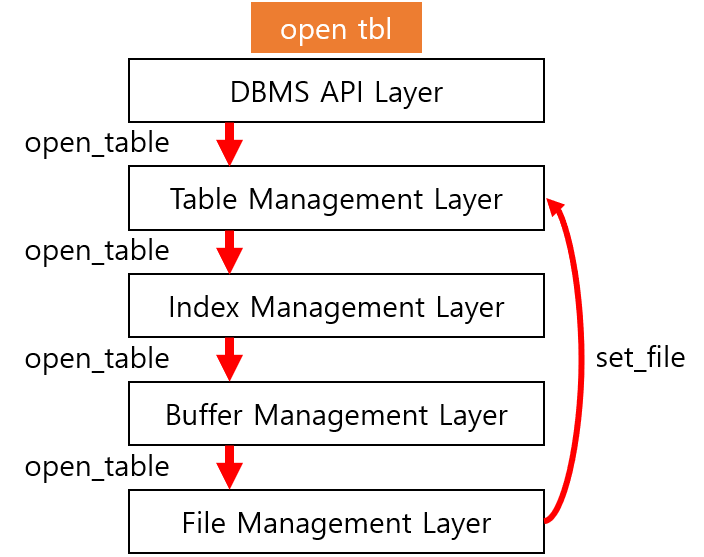
\includegraphics[width=0.48\linewidth]{images/dataflow/open_table.png}}
	\subfloat[]{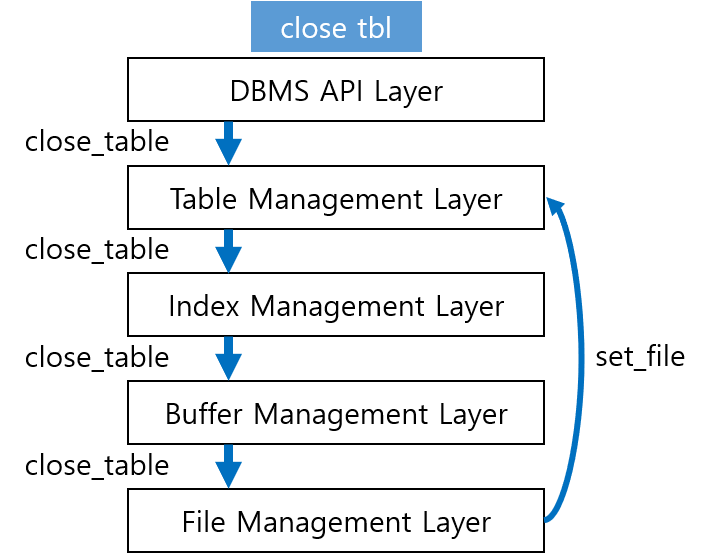
\includegraphics[width=0.48\linewidth]{images/dataflow/close_table.png}}
	\caption{Data flow in (a) open table and (b) close table}
\end{figure}


\subsubsection{Page Management}
\texttt{Index Management Layer}에서 insert, delete, update, find 연산을 수행할 때는 database file에 존재하는 page를 읽고 써야 한다. 또한 insert나 delete가 수행될 때는 page가 새로 생기거나 사라질 수도 있다. 이러한 모든 작업은 \texttt{File Management Layer}에서 수행되어야 하지만 효율을 위해 중간에 \texttt{Buffer Management Layer}를 두었기 때문에 \texttt{Index Management Layer}는 \texttt{File Management Layer}의 method를 직접 호출하기보다는 \texttt{Buffer Management Layer}의 method를 호출한 뒤, \texttt{Buffer Management Layer}가 \texttt{File Management Layer}의 method를 호출하게 함이 layered architecture violation을 막을 수 있다.

\paragraph{Page Read and Write}
\texttt{Index Management Layer}에서 page에 대해 읽고 쓰기 위해서는 우선 \texttt{Buffer Management Layer}에 (table id, page id)에 대응하는 page를 요청한다. 만약 해당하는 page가 caching 되어있지 않다면 \texttt{File Management Layer}에 해당 page를 요청한 뒤, \texttt{Index Management Layer}에 제공한다.

\begin{algorithm}
	\caption{Get page from Buffer Manager}
	\begin{algorithmic}
		\Function{BufferManager.GetPage}{table id, page id}
			\If {(table id, page id) $\notin$ BufferManager.Cache}
				\State BufferManager.Cache[table id, page id] = FileManager.GetPage(table id, page id)
			\EndIf
			
			\State \Return {BufferManager.Cache[table id, page id]}
		\EndFunction
	\end{algorithmic}
\end{algorithm}

만약에 해당 page가 수정되었다면 page를 요청한 곳에서 dirty flag를 set하여 이후 \texttt{Buffer Management Layer}가 해당 수정을 \texttt{File Management Layer}에게 전달할 수 있도록 한다.
정리하면 page에 관련된 write, read는 다음의 방식으로 처리된다.

\begin{algorithm}
	\caption{Case 1 - page를 읽기만 하는 경우}
	
	\hspace*{8pt} \textbf{Input}: table id, page id\\
	
	\begin{algorithmic}
		\State page = BufferManager.GetPage(table id, page id)
		
		\State doWork(page)
	\end{algorithmic}
\end{algorithm}

\begin{algorithm}
	\caption{Case 2 - page에 쓰기도 하는 경우}
	
	\hspace*{8pt} \textbf{Input}: table id, page id\\
	
	\begin{algorithmic}
		\State page = BufferManager.GetPage(table id, page id)
		
		\State doWork(page)
		
		\State page.dirty := True
	\end{algorithmic}
\end{algorithm}


\paragraph{Page Create and Free}
\texttt{Index Management Layer}가 새로운 page의 할당이 필요한 경우에는 해당 table의 database file에 free page가 있다면 해당 free page를 할당해준다. 그렇지 않다면 database file에 새로운 page에 대한 공간을 할당한다. 할당한 이후에 file header page를 수정하고, free page linked list를 수정하는 행위는 단순히 page에 write를 하는 것과 동일하므로 이러한 작업은 \texttt{Buffer Management Layer}에서 수행한다.


\end{document}